\chapter{Experimental Results}
\label{ch:results}

\section{Overview}

This chapter outlines the outcomes of the individual AS\textsuperscript{6} system blocks and evaluates their performance and realizability.  Since a large transition was made from original research and goals, many limitations were realized in the final prototype design presented in this thesis.  Feasibility was desired during the implementation stage of this work, causing this transition, but physical implementations were produced and analyzed.  Since certain channel conditions couldn't be replicated in reality baseline evaluations were produced for proof of concept, and rigorous hardening is a viable path for future work.\\ 

\section{Spectral Subtraction}

The goal of this section is to present the results of the Spectral Subtraction signal processing block.  This block, as mentioned in previous sections, tries to remove non-orthogonal known signals from the spectrum that are located on the same frequency of the desired signal.  Since the receiver is not allowed to move to other bands, this mimics the effects of a wide-band jamming system, causing all effective bandwidth or throughput to diminish.  From the theoretical simulations it is possible to remove the interfering signal but only under severe limitations or constraints.  The primary issue is that the signal is extremely time varying and alignment is quite difficult.  To be precise, this block tries to align a source signal with the received signal, and then subtract that signal from all future received segments. This alignment is difficult because the received signal is corrupted by noise and the channel which it passes through. That corruption is time varying as well, and difficult to model over many frames to provided sufficient signal removal.  In order to operate, this system assumes the interferer's system is completely known, including the data that is being modulated into the spectrum.  Therefore it is the goal of the Spectral Subtraction block is to regenerate the corruption caused by the channel, apply that to the source signal, and then subtract.  The experimental evaluation is outlined next and the analysis of its performance.\\

\subsection{Experiment}

This experiment consists of four USRP2 radio transceivers.  One radio acting as a transmitter, one the interferer, and two receive radio connected through a MIMO-USRP cable.  The cable causes direct synchronization between the receive radios.  This is required to perform maximal ratio combining to correctly align signals constructively.  During testing, the interferer first begins transmitting data, then the desired transmitter begins to transmit.  At all times the receiver is actively receiving all signals in the spectrum.  A sample of the combined received signals can be seen in Figure \ref{fig:combo_signal_time}.  The lower energy sections represent the individual signals and the high energy level sections show the mixed signals.\\


All transmissions utilize GMSK, due to its resilience to changes in the radio's power amplifier.  All radios operate at 100kbits/sec, well under the maximum rate of the radios, minimizing the load on the machines themselves and the amount of data generated.  The machines connected to the radios are all have Core Series Intel processors, installed with Ubuntu Linux 10.10 and 12.04.  All machines were also running MATLAB 2011B, and GNU-Radio 3.6.2git-145-g7c8347ca built from the git repository.  All signal recordings/reception was done in GNU-Radio and all signal processing at baseband was done in MATLAB.  Figure \ref{ss_setup_real} is a picture of the experimental setup with all four radios

\begin{figure}
\centering
\includegraphics[scale=0.1]{ss_setup_real.eps}
\caption{Spectral Subtraction Hardware Setup}
\label{ss_setup_real}
\end{figure}

\subsection{Analysis}

The system was able to correctly identify power changes in the signal and provide the most accurate estimates before the signals begin to mix.  This mixing of signals cannot last for long periods of time because the non-idealities of the hardware and environment begin to corrupt the estimate of the interfering signal.  This corruption removed any hope of desired signal recovery.  The corruption can be seen clearly in Figure \ref{ss_oscillation}, as the frames further from the estimate become more and more corrupted.  This period of time for which the estimate provides enough accuracy for spectral removal depends on the changes in phase frequency and channel effects.\\

Many of the non-idealities associated with Spectral Subtraction were discussed in the Implementation chapter.  Though most of effort was put towards compensating for these effects, they still produced a large amount of error in the final design.  These sources of corruption manifested as several different errors in the output of the block.  The first was timing offsets.  Since the interferer is extremely time-varying, if a single bit is missed, the entire signal downstream becomes corrupted.  If this timing is out of phase \(\pi\) radians, then an identical corruption occurs.  As the phase offset \(\phi\) is removed, this exponentially decreases the error.  As for carrier frequency and phase offsets, this error manifests as an oscillating error in the output signal.  Figure \ref{ss_oscillation} shows severals frames and the resulting energy left behind after subtraction.  This plot was generate by a simplified test, just the interferer transmitted data and attempts were made to nullify these transmissions.  These oscillations point towards problems in phase or frequency estimations.\\

\begin{figure}
\centering
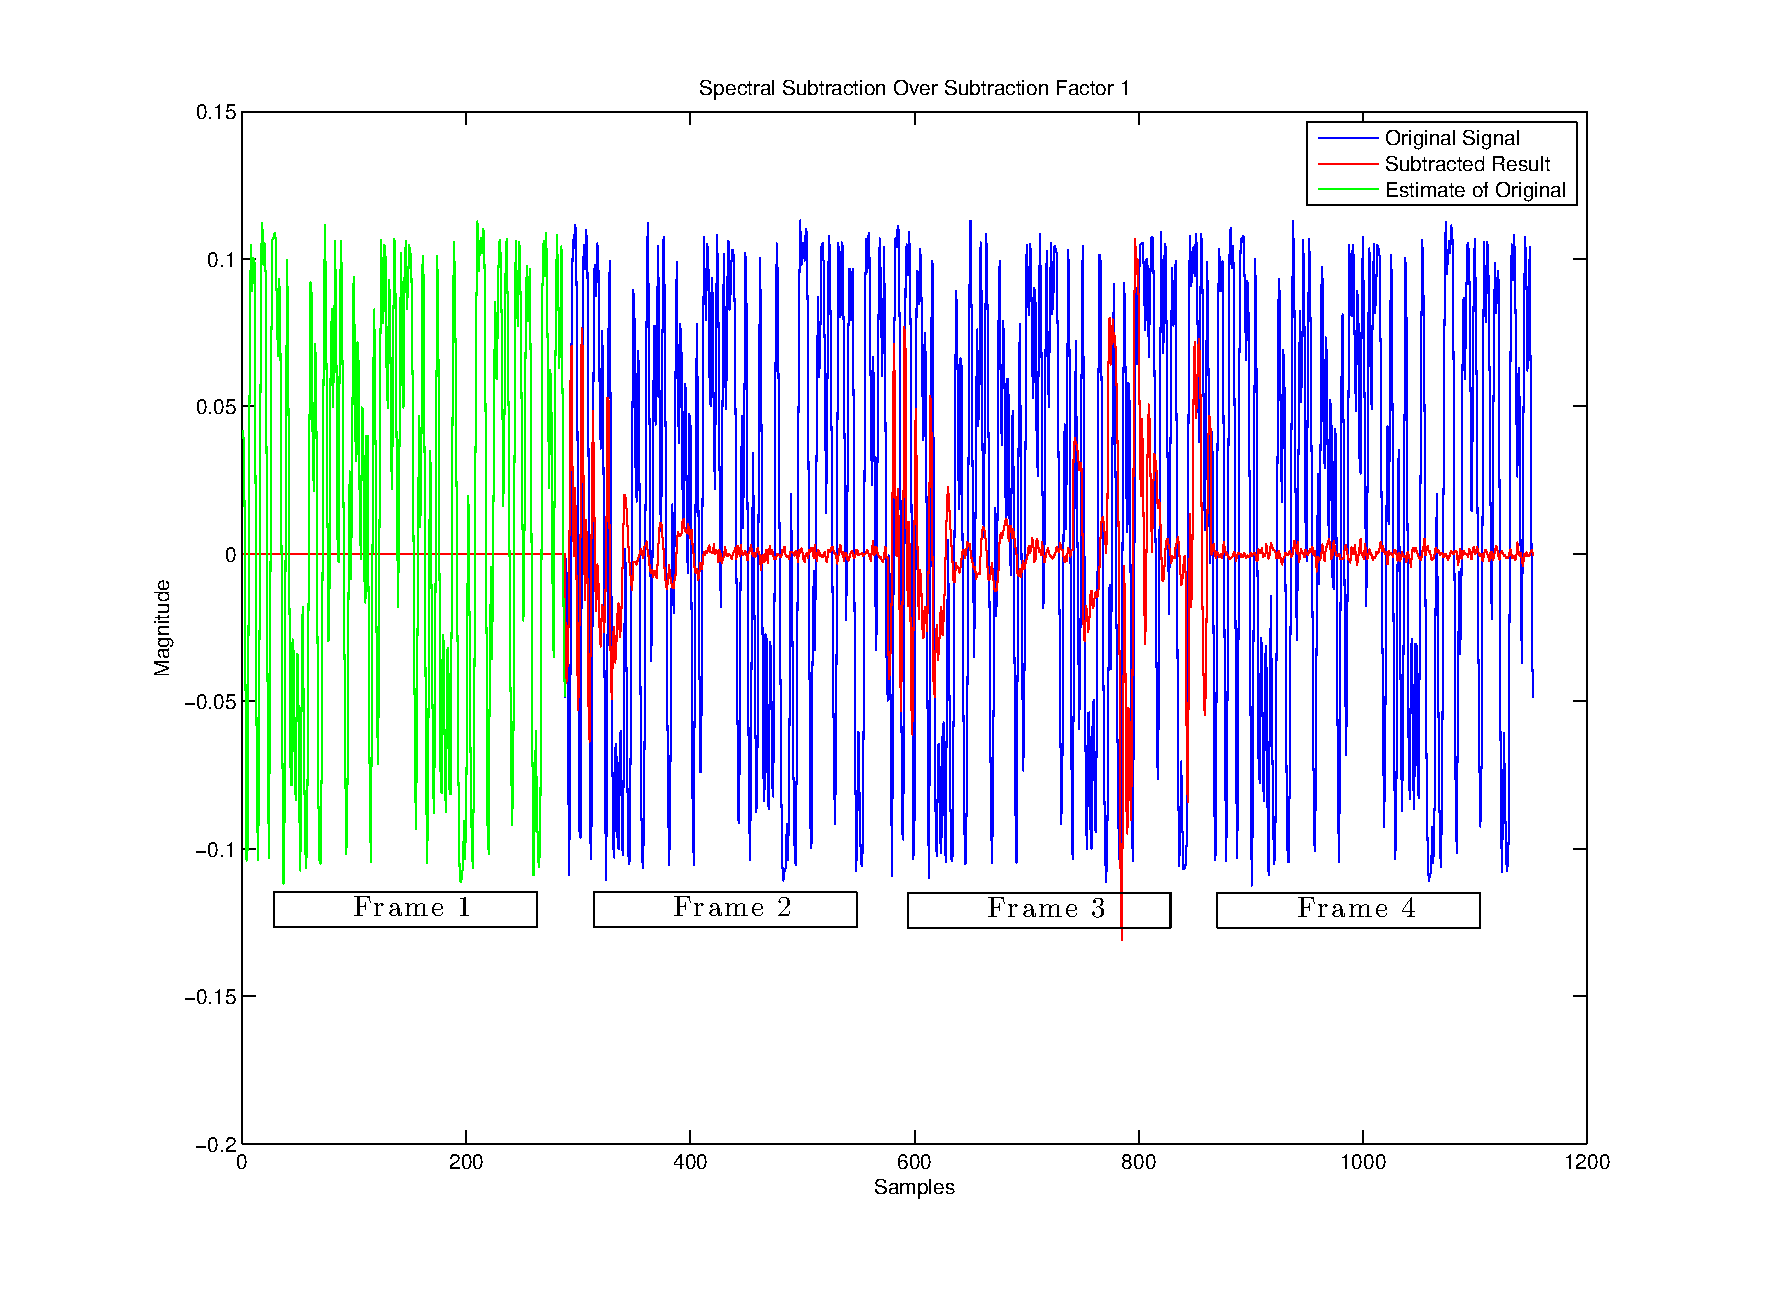
\includegraphics[scale=0.5]{ss_oscillation.eps}
\caption{After Spectral Subtraction the error, or the remaining not removed interferer, appears as an oscillation at the remaining frame positions.  Green represents the subtraction frame estimate, blue the originally received frames, and red the frames after subtraction.}
\label{ss_oscillation}
\end{figure}


%%To evaluate the Spectral Subtraction block the signal was demodulated, timing recovered, and compared against the transmitted data.  Mueller Muller timing was used as a timing recovery method.  Several runs were made, and varying results were recorded.  Even with perfect knowledge of the exact modulated data, the corruption caused by the environment proved extremely hazarous to the signal.  Since the frequency drift of the USRP2 crystal oscillators, which control the transmission and reception frequencies, can vary on the order of kilohertz.  %%
These non-ideality seemed to be the most difficult problem to compensated for, and become worse when the signals are mixed.  This is because they cannot be directly measured.  A oscillating error in the spectrum, shown in Figure \ref{ss_oscillation}, mirror the effects shown in the simpler nullifying case.  As express previously, Spectral Subtraction is very susceptible to data corruption.  It is analogous to hitting a moving target, since the operation is extremely time varying and time dependent.\\  

To help compensate for these non-idealities phase synchronization and carrier synchronization was attempted with the received signal.  As outlined in the Implementation chapter, Spectral Subtraction is designed as a receiver in a receiver system.  The front received locks onto the interferer, applies necessary phase shifts, and subtracts a synthetically generated signal from the previously known data which has also been modulated and pulse-shaped.  Unfortunately this the received data also contains many other effects cause by the channel, including multi-path and large amounts of noise.  To resolve this the front receiver must estimate the channel and apply the same amount of noise to the signal to remove it sufficiently.  With \(H_{I}\) and \(H_{D}\) representing the interferer's channel and desired signal's channel respectively.  The transmitted symbols of the desire signal \(\bf{x}_{D}\) and the interferer \(\bf{x}_{I}\).  The received signal can be written as: \( \bf{y}=H_{I}^\textit{H}x_{I}+H_{D}^\textit{H}x_{D}+w \).  Only \(\bf{x_{I}}\) is known in this realization, and both \(\bf{H_{I}}\) and \(\bf{w}\) are time dependent.  As mentioned previously SS is very susceptible to any carrier, power, and timing effects.\\


It is important to show Spectral Subtraction operating correctly and when errors occur in the estimation.  Figure \ref{ss_result_great} show a desired result from Spectral subtraction when all timing is aligned, while Figure \ref{ss_result_bad} shows the error propagation through the frames.  Both these results looked 20 frames ahead of the section used for subtraction.  Finally Figure \ref{many_frames}, shows the error associated with increasing the frames looking ahead.  As expected, the further you move away from your original subtraction frame, the worse your results become.\\

\begin{figure}
\centering
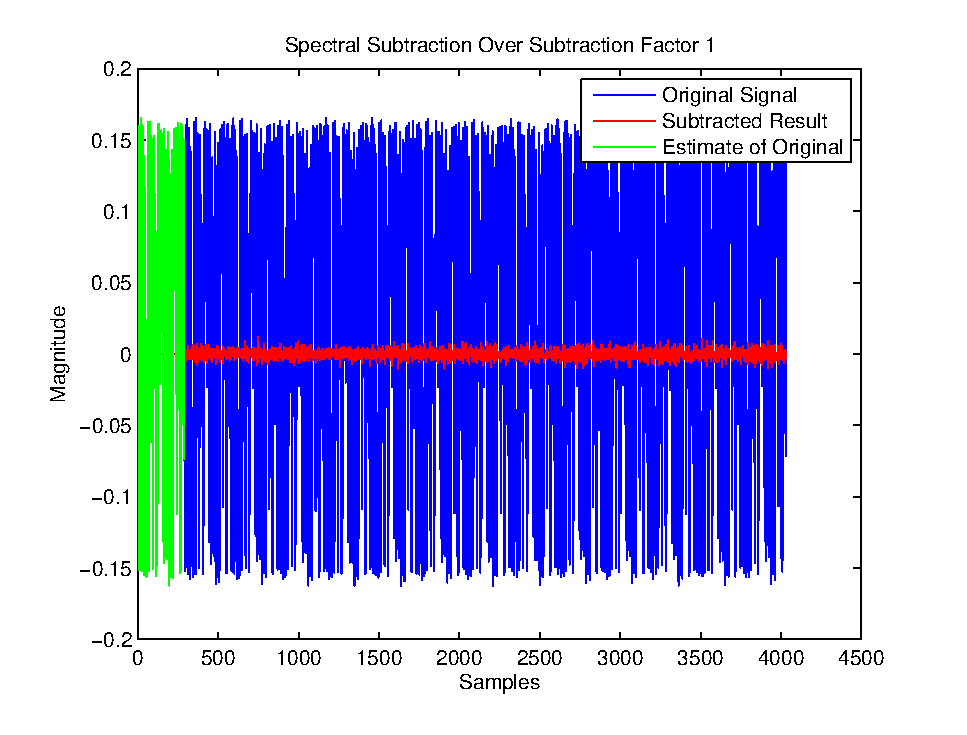
\includegraphics[scale=0.7]{ss_result_GREAT.eps}
\caption{Desired result after Spectral Subtraction with 20 forward frames, producing limited residual signal.  Phase changes minimally across these frames.}
\label{ss_result_great}
\end{figure}

\begin{figure}
\centering
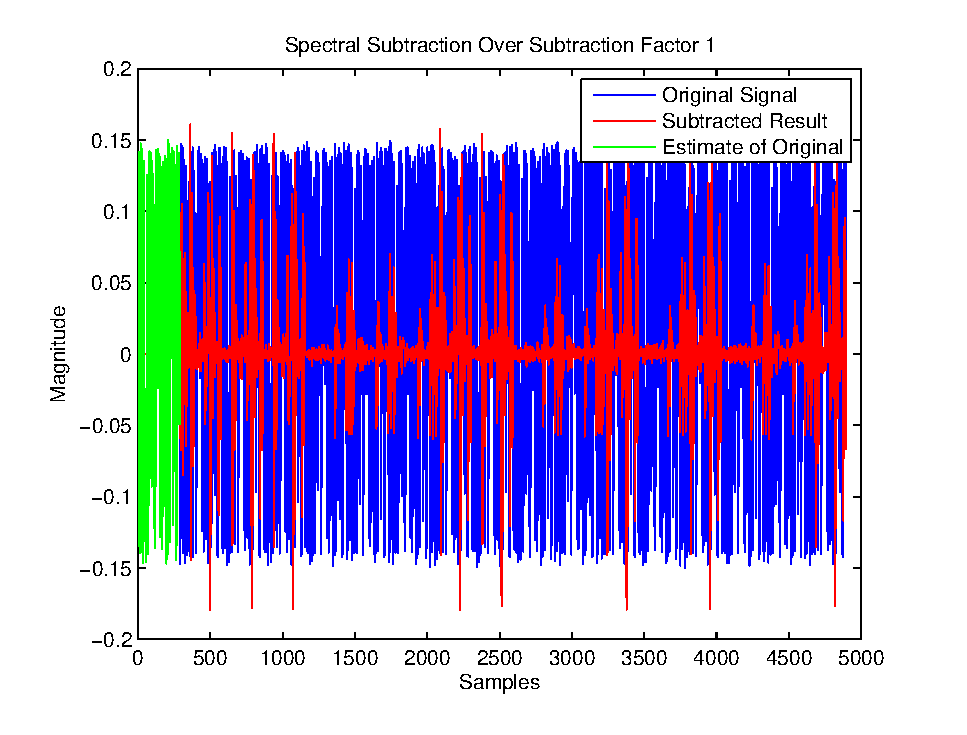
\includegraphics[scale=0.7]{ss_result_BAD_Timing.eps}
\caption{Error after Spectral Subtraction with incorrect phase estimates with 20 forward frames.  The error oscillates among the remaining frames.}
\label{ss_result_bad}
\end{figure}

\begin{figure}
\centering
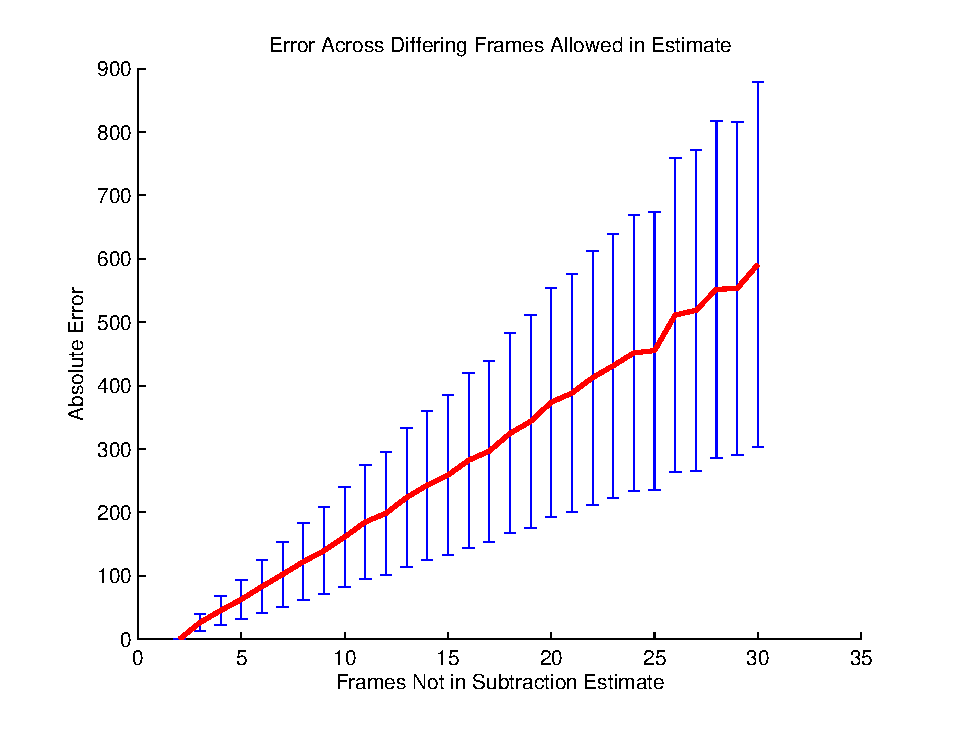
\includegraphics[scale=0.7]{many_frames.eps}
\caption{Error associated with increasing duration between restimation of subtractions frames.  The far the subtraction pushed into future frames, the more inaccurate that estimate becomes.}
\label{many_frames}
\end{figure}


%Since noise couldn't be varied in this implementation for direct comparision against simulation, presented is a series of runs and their coinciding errors.  Each run only represents the periods for which the signals are mixed, which is roughly 3 seconds.  The error represents the accuracy of the demodulated signal and not the amount of unwanted still existing in the channel, since it is less desired.  This data can be seen in figure \ref{ss_error_runs}.\\

%\begin{figure}\label{ss_error_runs}
%\includegraphics{ss_error_runs.eps}
%\end

\subsection{Summary}

Spectral Subtraction in a extremely well studied area in signal processing, but no existing literature exists for its application in a digital communication system.  It has been shown here that it can be quite difficult for it to be applied, even under strict constraints.  Under the conditions of this thesis, the assumptions are quite reasonable, but due to the large amount of error in the results, more may need to be considered.  These may include accuracy requirements for physical equipment, primarily to reduce carrier frequency drift.  Burst scenarios may also be considered to reduce bit error rate.  Overall, for a completely non-existent field of study, these results point the possibility of operational success.  Future work will we required, especially during the implementation phase of designs.\\

\section{Signal Separation}

The Signal Separation block changed the most from the original research design.  Much of the design needed to be reconsidered because of time constraints and lack of robust research conclusions.  The design distilled down to a combination of Maximal Ratio Combining and adaptive equalization.  Two well know concepts in communication system design, and rather straight forward to implement.  Maximal Ratio Combining provides the benefits of maximizing the spectrum spatially, while also adaptively equalizing these separated data streams to help remove corruption left over by spectral subtraction of the channel itself.  The more dimensionality that can be exploited the more performance can be extracted.\\

\subsection{Experiment}

Signal Separation utilized an identical setup as the Spectral Subtraction testing, which is quite obvious since Signal Separation is downstream from Spectral subtraction in the data path.  The interferer was also removed from this testing, and the noise that pre-existed in the spectrum used to reflect the noise remaining from Spectral Subtraction.  This decision was made to separate problems or issues with the performance of the Spectral Subtraction block, providing direct analysis and evaluation of the Signal Separation block.  It takes in two data stream, which have been timing synchronize through the use of the MIMO USRP cable.  These streams are equalized by an LMS Adaptive equalizer of length 14.  These taps provided the Maximal Ratio Combining weight analysis, providing information on which of the channel was less corrupted.  This is done by combining the filter tap values and taking the ratio of the two equalizers, and these weights determine how much of each signal is added to the final output signal.\\ 

Again all transmissions utilize GMSK, due to its resilience to changes in the radio's power amplifier.  All radios operate at 100kbits/sec, well under the maximum rate of the radios, minimizing the load on the machines themselves and the amount of data generated.  The machines connected to the radios are all Core Series Intel processing, installed with Ubuntu Linux 10.10 and 12.04.  All machines were also running MATLAB 2011B, and GNU-Radio 3.6.2git-145-g7c8347ca built from the git repository.  All signal recordings/reception was done in GNU-Radio and all signal processing at baseband was done in MATLAB.  Therefore the entire Signal Separation block resides in MATLAB.\\  

Several separate transmissions were made and baseline bit error rates were calculated.  This was done by quantizing the final output and comparing the results.  The Mueller Muller method again was used for timing recovery due to its robustness.  It doesn't account for bit slips, but due to the rather short periods of transmission these can be ignored.  Since this block is designed to help in rather noisy and localized corruption situations, it can be very hard to test because there is no control over the spectral environment to set such conditions.  Rather this design shows a proof of concept with SDR technology.  The results for the baseband tests are shown in Figure \ref{ssep_snr_tests}.\\

%\begin{figure}\label{ssep_results}
%\includegraphics{ssep_results.eps}
%\caption{Implementation Signal Separation Performance with varying TX gain}
%\end{figure}

\subsection{Analysis}

From the results seen from the baseline testing, reception seems to be quite reasonable given the inferior hardware. To provide a comparison to the simulated results, the transmitter power was lowered to synthetically reduce the SNR of the signal.  The results of these tests can be seen in Figure \ref{ssep_snr_tests}.   

\begin{figure}[!ht]
\centering
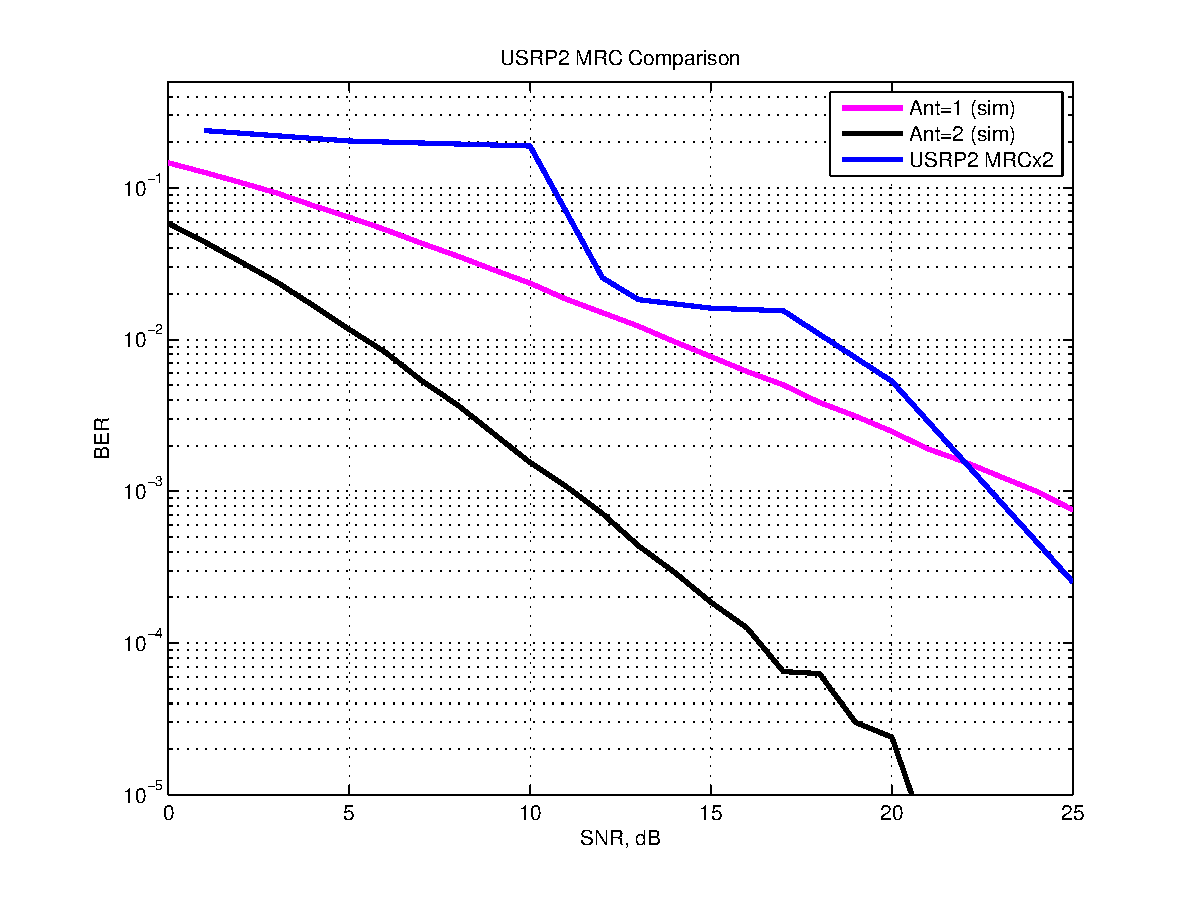
\includegraphics[scale=0.5]{mrc_snr_comp.eps} %{ssep_snr_tests.eps}
\caption{Signal Separation MRC performance comparison against simulations.  Each data point represents the average BER of 67,000 frames received at varying SNR levels.}
\label{ssep_snr_tests}
\end{figure}

Since only antennas are provided by the AntSS block, MRC will suffer.  Higher performance will be provided by more input signals, but that would increase the complexity of the system significantly.  More input signals could be a future alley for BLISS system for future research.  For the current system architecture the results are acceptable given the limitations and variability in the hardware itself.\\


\section{Summary}

These results show that it is extremely difficult to avoid a wide-band jammer even when fine details are known about the interferer itself.  Spectral Subtraction has large downfalls in its implemented realization due to its fragile nature.  Small non-idealities can cause large errors, especially in timing, causing a large misalignment in the subtracted signal.  Equipment with higher tolerances would be a way of minimizing these effects.  Signal Separation is focused in solid theoretical foundation and provides additional SNR above single antenna reception, allowing an extrapolation in the dimensionality of the environment and the signal itself.  It was fully implemented with reasonable BER given the non-ideal hardware.  Additional antennas should be considered for further gains from Maximal Ratio Combining.\\




